% \documentclass[pscyr,specification,annotation]{itmo-student-thesis}
\documentclass[pscyr]{itmo-student-thesis}

%% Опции пакета:
%% - specification - если есть, генерируется задание, иначе не генерируется
%% - annotation - если есть, генерируется аннотация, иначе не генерируется
%% - pscyr - делает все шрифтом Times New Roman, требует пакета pscyr.
%% - times - делает все шрифтом Times New Roman, собирается с помощью xelatex

\usepackage{graphicx}
\graphicspath{{logo/}{pics/}}

%% Делает запятую в формулах более интеллектуальной, например:
%% $1,5x$ будет читаться как полтора икса, а не один запятая пять иксов.
%% Однако если написать $1, 5x$, то все будет как прежде.
\usepackage{icomma}

%% Один из пакетов, позволяющий делать таблицы на всю ширину текста.
\usepackage{tabularx}

%% Данные пакеты необязательны к использованию в бакалаврских/магистерских
%% Они нужны для иллюстративных целей
%% Начало
\usepackage[russian]{cleveref}
\usepackage{tikz}
\usepackage{csvsimple}
\usetikzlibrary{arrows}
\usepackage{filecontents}
\usepackage{booktabs}
\addbibresource{thesis.bib}

\usepackage{pgfplots, pgfplotstable}
\usepgfplotslibrary{fillbetween}
\pgfplotsset{compat=newest}

\makeatletter
\pgfplotsset{%
    /pgfplots/flexible xticklabels from table/.code n args={3}{%
        \pgfplotstableread[#3]{#1}\coordinate@table
        \pgfplotstablegetcolumn{#2}\of{\coordinate@table}\to\pgfplots@xticklabels
        \let\pgfplots@xticklabel=\pgfplots@user@ticklabel@list@x
    }
}
\makeatother%
\definecolor{basicno}{rgb}{0.624,0.0,0.0}
\definecolor{basicsome}{rgb}{0.424,0.0,0.0}
\definecolor{random}{rgb}{0.0,0.100,0.424}
\definecolor{gena}{rgb}{0.0,0.100,0.624}
\definecolor{heuno}{rgb}{0.2,0.524,0.2}
\definecolor{heusome}{rgb}{0.2,0.424,0.2}
\definecolor{heumore}{rgb}{0.1,0.324,0.1}

\newcommand{\addplottime} [2] {%
\addplot 
    [color=#2, fill=#2, fill opacity=0.33]
    plot [error bars/.cd, error bar style={line width=1pt}, y dir = both, y explicit]
    table[x expr=\coordindex, y=mean_time, y error=std_time]{#1};
}

\newenvironment{timeaxis} [3] {%
\begin{axis}[
    enlarge x limits=0.2,
    ybar=0pt, 
    width=#1,
    height=#2,
    bar width=8pt,
    ymin=0,
    xlabel=Датасет,
    ylabel=Время работы в сек,
    flexible xticklabels from table={#3}{algo}{col sep=comma},
    xticklabel style={text height=1.5ex, font=\tiny}, % To make sure the text labels are nicely aligned
    xtick=data,
    legend cell align={left},
    % legend style={at={(0.02,0.98)},anchor=north west},
]
}{%
\end{axis}
}

\newcommand{\timebig} [2] {%
\pgfplotstableread[col sep=comma]{../data/big/basic-00.csv}\basicno
\pgfplotstableread[col sep=comma]{../data/big/basic-05.csv}\basicsome
\pgfplotstableread[col sep=comma]{../data/big/heuristic-00.csv}\heuno
\pgfplotstableread[col sep=comma]{../data/big/heuristic-05.csv}\heusome
\pgfplotstableread[col sep=comma]{../data/big/heuristic-15.csv}\heumore
\pgfplotstableread[col sep=comma]{../data/big/random.csv}\random

\begin{tikzpicture}
\begin{timeaxis}{#1}{#2}{../data/big/heuristic-15.csv}

\addplottime{\basicno}{basicno}
\addplottime{\basicsome}{basicsome}
\addplottime{\random}{random}
\addplottime{\heuno}{heuno}
\addplottime{\heusome}{heusome}
\addplottime{\heumore}{heumore}

\legend{%
    Ветви/границы, 
    Ветви/границы с $<5\%$, 
    Случайный, 
    Ветви/границы + эвристика, 
    Ветви/границы + эвристика с $<5\%$, 
    Ветви/границы + эвристика с $<15\%$ 
}

\end{timeaxis}
\end{tikzpicture}
}

\newcommand{\timeeasy} [2] {%
\pgfplotstableread[col sep=comma]{../data/easy/basic-00.csv}\basicno
\pgfplotstableread[col sep=comma]{../data/easy/basic-05.csv}\basicsome
\pgfplotstableread[col sep=comma]{../data/easy/heuristic-00.csv}\heuno
\pgfplotstableread[col sep=comma]{../data/easy/heuristic-05.csv}\heusome
\pgfplotstableread[col sep=comma]{../data/easy/heuristic-15.csv}\heumore
\pgfplotstableread[col sep=comma]{../data/easy/random.csv}\random

\begin{tikzpicture}
\begin{timeaxis}{#1}{#2}{../data/easy/heuristic-15.csv}

\addplottime{\basicno}{basicno}
\addplottime{\basicsome}{basicsome}
\addplottime{\random}{random}
\addplottime{\heuno}{heuno}
\addplottime{\heusome}{heusome}
\addplottime{\heumore}{heumore}

\legend{%
    Ветви/границы, 
    Ветви/границы с $<5\%$, 
    Случайный, 
    Ветви/границы + эвристика, 
    Ветви/границы + эвристика с $<5\%$, 
    Ветви/границы + эвристика с $<15\%$ 
}

\end{timeaxis}
\end{tikzpicture}
}

\newcommand{\timetrees} [2] {%
\pgfplotstableread[col sep=comma]{../data/trees/basic-00.csv}\basicno
\pgfplotstableread[col sep=comma]{../data/trees/basic-05.csv}\basicsome
\pgfplotstableread[col sep=comma]{../data/trees/heuristic-00.csv}\heuno
\pgfplotstableread[col sep=comma]{../data/trees/heuristic-05.csv}\heusome
\pgfplotstableread[col sep=comma]{../data/trees/heuristic-15.csv}\heumore
\pgfplotstableread[col sep=comma]{../data/trees/random.csv}\random

\begin{tikzpicture}
\begin{timeaxis}{#1}{#2}{../data/trees/heuristic-15.csv}

% \addplottime{\basicno}{basicno}
% \addplottime{\basicsome}{basicsome}
\addplottime{\random}{random}
\addplottime{\heuno}{heuno}
\addplottime{\heusome}{heusome}
\addplottime{\heumore}{heumore}

\legend{%
    % Ветви/границы, 
    % Ветви/границы с $<5\%$, 
    Случайный, 
    Ветви/границы + эвристика, 
    Ветви/границы + эвристика с $<5\%$, 
    Ветви/границы + эвристика с $<15\%$ 
}

\end{timeaxis}
\end{tikzpicture}
}

\newcommand{\addploterror}[2] {% 
\addplot 
    [color=#2, fill=#2, fill opacity=0.33]
    plot [error bars/.cd, error bar style={line width=1pt}, y dir = both, y explicit] 
    table[x expr=\coordindex, y=mean_error, y error=std_error]{#1}; 
}

\newenvironment{erroraxis}[2] {% 
\begin{axis}[
    ytick={0,0.1,...,0.9},
    enlarge x limits=0.2,
    ybar=0pt, 
    width=#1,
    height=#2,
    bar width=8pt,
    ymin=0,
    xlabel=Датасет,
    ylabel=Отоносительная погрешность,
    flexible xticklabels from table={../data/easy/heuristic-15.csv}{algo}{col sep=comma},
    xticklabel style={text height=1.5ex, font=\tiny}, % To make sure the text labels are nicely aligned
    xtick=data,
    legend style={at={(0.02,0.98)},anchor=north west},
]
}{%
\end{axis}
}

\newcommand{\errorbig}[2] {%
\pgfplotstableread[col sep=comma]{../data/extra/heuristic-05.csv}\heusome
\pgfplotstableread[col sep=comma]{../data/extra/heuristic-15.csv}\heumore
\pgfplotstableread[col sep=comma]{../data/extra/random.csv}\random

\begin{tikzpicture}
\begin{erroraxis}{#1}{#2}

\addploterror{\random}{random} 
\addploterror{\heusome}{heusome}
\addploterror{\heumore}{heumore}

\legend{%
    Случайный, 
    Эвристика с $<5\%$, 
    Эвристика с $<15\%$ 
}

\end{erroraxis}
\end{tikzpicture} 
}

\newcommand{\erroreasy}[2] {%
\pgfplotstableread[col sep=comma]{../data/easy/basic-05.csv}\basicsome
\pgfplotstableread[col sep=comma]{../data/easy/heuristic-05.csv}\heusome
\pgfplotstableread[col sep=comma]{../data/easy/heuristic-15.csv}\heumore
\pgfplotstableread[col sep=comma]{../data/easy/random.csv}\random

\begin{tikzpicture} 
\begin{erroraxis}{#1}{#2}

\addploterror{\basicsome}{basicsome}
\addploterror{\random}{random}
\addploterror{\heusome}{heusome}
\addploterror{\heusome}{heumore}

\legend{%
    Перебор с $<5\%$, 
    Случайный, 
    Эвристика с $<5\%$, 
    Эвристика с $<15\%$ 
}

\end{erroraxis}
\end{tikzpicture}
}

\newcommand{\errortimeaddplot}[2] {%
\addplot 
    [scatter, color=#2, style={ultra thick}] 
    table[x=algo, y=mean_time]{#1};
\addplot 
    [name path=upper, color=#2] 
    table[x=algo, y expr=\thisrow{mean_time}-\thisrow{std_time}]{#1};
\addplot 
    [name path=lower, color=#2] 
    table[x=algo, y expr=\thisrow{mean_time}+\thisrow{std_time}]{#1};
\addplot 
    [fill, fill opacity=0.2, color=#2] 
    fill between[of=upper and lower];
}

\newcommand{\errortotime}[2] {%
\pgfplotstableread[col sep=comma]{../data/datasets/time_to_error/diabetes70-None.csv}\diabet
\pgfplotstableread[col sep=comma]{../data/datasets/time_to_error/kin8nm30-None.csv}\kinmerrtime
% \pgfplotstableread[col sep=comma]{../data/datasets/time_to_error/house_8L37-None.csv}\house

\begin{tikzpicture}
\begin{axis}[
    xtick={0.00,0.05,0.10,0.15,0.20,0.25},
    x tick label style={/pgf/number format/.cd,
            fixed, fixed zerofill, precision=2, /tikz/.cd},
    enlarge x limits=0.2,
    width=#1,
    height=#2,
    ymin=0,
    xlabel=Заданная допутсимая погрешность алгоритма,
    ylabel=Время работы в сек.,
    scatter/classes={a={mark=o}},
]

\errortimeaddplot{\diabet}{heusome}
\errortimeaddplot{\kinmerrtime}{basicno}
% \errortimeaddplot{\house}{random}

\legend{%
    diabetes-70 деревьев,,,,
    kin8nm-30 деревьев,,,,
    house\_8L-37 деревьев,
}

\end{axis}
\end{tikzpicture}
}

\newcommand{\addplotsmac}[5] {%
\addplot 
    [scatter, color=#2]
    plot [error bars/.cd, error bar style={line width=1pt}, y dir = both,
    y explicit] table[x index=#3, y expr=1-\thisrow{#4}, y error index=#5]{#1}; 
}

\newcommand{\smacsize} [2] {%
\pgfplotstableread[col sep=comma, header=false]{../data/smac/limits/new_iris_forest.csv}\forestiris
\pgfplotstableread[col sep=comma, header=false]{../data/smac/limits/new_iris_random.csv}\randomiris
\pgfplotstableread[col sep=comma, header=false]{../data/smac/limits/new_leter_forest.csv}\forestletter
\pgfplotstableread[col sep=comma, header=false]{../data/smac/limits/new_leter_random.csv}\randomletter
\pgfplotstableread[col sep=comma, header=false]{../data/smac/limits/new_gina_forest.csv}\forestgina
\pgfplotstableread[col sep=comma, header=false]{../data/smac/limits/new_gina_random.csv}\randomgina

\begin{tikzpicture}
\begin{axis}[
    enlarge x limits=0.2,
    width=#1,
    height=#2,
    ymin=0,
    xlabel=Размер пространства гиперпараметров,
    ylabel=Оценка точности,
    xtick=data,
    scatter/classes={a={mark=o}},
    legend style={at={(1.02,0.98)},anchor=north west},
]

\addplotsmac{\forestiris}{heusome}{2}{4}{5}
\addplotsmac{\forestletter}{basicsome}{2}{4}{5}
\addplotsmac{\forestgina}{gena}{2}{4}{5}
\addplotsmac{\randomiris}{heuno}{2}{4}{5}
\addplotsmac{\randomletter}{basicno}{2}{4}{5}
\addplotsmac{\randomgina}{random}{2}{4}{5}

\legend{%
    iris,
    leter,
    gina-agnositc,
}

\end{axis}
\end{tikzpicture}
}

\newcommand{\smaccount} [2] {%
\pgfplotstableread[col sep=comma, header=false]{../data/smac/runcount/iris_forest.csv}\forestiris
\pgfplotstableread[col sep=comma, header=false]{../data/smac/runcount/iris_random.csv}\randomiris
\pgfplotstableread[col sep=comma, header=false]{../data/smac/runcount/leter_forest.csv}\forestletter
\pgfplotstableread[col sep=comma, header=false]{../data/smac/runcount/leter_random.csv}\randomletter
\pgfplotstableread[col sep=comma, header=false]{../data/smac/runcount/gina_forest.csv}\forestgina
\pgfplotstableread[col sep=comma, header=false]{../data/smac/runcount/gina_random.csv}\randomgina

\begin{tikzpicture}
\begin{axis}[
    enlarge x limits=0.2,
    width=#1,
    height=#2,
    ymin=0,
    xlabel=Количество запусков целевого алгоритма,
    ylabel=Оценка точности,
    xtick=data,
    scatter/classes={a={mark=o}},
    legend style={at={(1.02,0.98)},anchor=north west},
]
\addplotsmac{\forestiris}{heusome}{0}{3}{4}
\addplotsmac{\forestletter}{basicsome}{0}{3}{4}
\addplotsmac{\forestgina}{gena}{0}{3}{4}
\addplotsmac{\randomiris}{heuno}{0}{3}{4}
\addplotsmac{\randomletter}{basicno}{0}{3}{4}
\addplotsmac{\randomgina}{random}{0}{3}{4}

\legend{%
    iris,
    leter,
    gina-agnositc,
}

\end{axis}
\end{tikzpicture}
}

\pgfplotstableread[col sep=comma, header=false]{../data/smac/forest.csv}\forest
\pgfplotstableread[col sep=comma, header=false]{../data/smac/random.csv}\random

\begin{tikzpicture}
\begin{axis}[
    only marks,
    enlarge x limits=0.01,
    % ybar=0pt, 
    width=\graphwidth,
    height=\graphheight,
    % bar width=8pt,
    ymin=0,
    xlabel=Random Forest \hspace{3em} Decision Tree \hspace{3em} SGD \hspace{1em}.,
    ylabel=обратная оценка точности,
    xticklabel style={text height=1.5ex, font=\tiny}, % To make sure the text labels are nicely aligned
    xtick=data,
    scatter/classes={a={mark=o}},
]
\addplot 
    [scatter, color=heuno]
    plot [error bars/.cd, error bar style={line width=1pt}, y dir = both, y explicit]
    table[x expr=\coordindex, y index=3, y error index=4]{\random};
\addplot 
    [scatter, color=basicno]
    plot [error bars/.cd, error bar style={line width=1pt}, y dir = both, y explicit]
    table[x expr=\coordindex, y index=3, y error index=4]{\forest};

\legend{%
    Оригинал, 
    Модификация,
}

\end{axis}
\end{tikzpicture}


\begin{document}
  
\studygroup{M3439}
\title{Оптимизация функции, задаваемой регрессионным лесом}
\author{Ягламунов Владислав Радикович}{Ягламунов В.Р.}
\supervisor{Фильченков Андрей Александрович}{Фильченков А.А.}{доцент, к.ф.-м.н.}{}
\publishyear{2019}
%% Дата выдачи задания. Можно не указывать, тогда надо будет заполнить от руки.
% \startdate{01}{сентября}{2018}
%% Срок сдачи студентом работы. Можно не указывать, тогда надо будет заполнить от руки.
% \finishdate{31}{мая}{2019}
%% Дата защиты. Можно не указывать, тогда надо будет заполнить от руки.
% \defencedate{15}{июня}{2019}

% \addconsultant{Белашенков Н.Р.}{канд. физ.-мат. наук, без звания}
% \addconsultant{Беззубик В.В.}{без степени, без звания}

\secretary{Павлова О.Н.}

%% Задание
%%% Техническое задание и исходные данные к работе
\technicalspec{Требуется разработать алгоритм поиска областей минимума
и максимума в данном обученном случайном регрессионном лесе. Требуется
минимизировать время работы алгоритма. Алгоритм должен возвращать точный ответ
или ответ отличающийся от точного не более чем не заданную величину. }

%%% Содержание выпускной квалификационной работы (перечень подлежащих разработке вопросов)
\plannedcontents{Описание существующих решений для оптимизации функции,
задаваемой регрессионным лесом. Разработка и реализация различных алгоритмов,
решающих поставленную задачу. Сравнение разработанных алгоритмов между собой
и существующими решениями задачи. }

%%% Исходные материалы и пособия
\plannedsources{}

%%% Цель исследования
\researchaim{Разработка эффективного алгоритма оптимизации функции, заданной регрессионным лесом.}

%%% Задачи, решаемые в ВКР
\researchtargets{\begin{enumerate}
    \item реализация интерфейса для работы с обученным случным регрессионным лесом;
    \item разработка алгоритмов оптимизации функции;
    \item интеграция разработанного алгоритма оптимизации случайного леса в существующие алгоритмы
    \item разработка тестирующей системы для алгоритмов оптимизации, позволяющей автоматическое
    тестирование на различных выборках и с набором заданных параметров;
    \item сравнение и анализ работы разработанных алгоритмов, сопоставление
    с существующими решениями.
    \end{enumerate}}

%%% Использование современных пакетов компьютерных программ и технологий
\addadvancedsoftware{%
    Язык программирования \texttt{C++}, для реализации алгоритма оптимизации
}{**todo: ref**}
\addadvancedsoftware{%
    Язык программирования \texttt{Python}, для тестирования и работы с машинным обучением
}{**todo: ref**}
\addadvancedsoftware{%
    Пакет \texttt{scikit-learn} с реализацией современных алгоритмов машинного обучения на языке \texttt{Python}
}{**todo: ref**}
\addadvancedsoftware{%
    Пакеты \texttt{automl: SMAC и random\_forest\_run}, для сравнительного анализа
}{**todo: ref**}

%%% Краткая характеристика полученных результатов
\researchsummary{Получен алгоритм для нахождения оптимума функции, заданной
случным регрессионным лесом, с возможностью настройки необходимой точности,
а также ограничения области поиска.}

%%% Гранты, полученные при выполнении работы
\researchfunding{При выполнении работы грантов получено не было.}

%%% Наличие публикаций и выступлений на конференциях по теме выпускной работы
\researchpublications{Отсутствуют.}

%% Эта команда генерирует титульный лист и аннотацию.
\maketitle{Бакалавр}

%% Оглавление
\tableofcontents

%% Макрос для введения. Совместим со старым стилевиком.
\startprefacepage

Существует множество алгоритмов, использующих суррогатные функции для
аппроксимации или предсказания различных процессов. Случайный регрессионный лес
часто может применяться в качестве такой функции, так как одно из его
положительных качеств --- возможность эффективно пересчитывать лес при
добавлении новой информации. Так на пример, случайный лес может использоваться
в качестве регрессионной модели для реализации алгоритмов последовательной
оптимизации основанной на модели (Sequential Model-Based Optimization ---
SMBO\cite{smac}) Однако, функция заданная таким образом является трудно обратимой
и сейчас не существует эффективных алгоритмов оптимизации и на практике
применяются не оптимальные алгоритмы, как, например, перебор случайных точек
пространства или локальный поиск.

%% Начало содержательной части.

\chapter{Описание предметной области и анализ существующих решений}

\section{Дерево принятия решений}

Дерево принятия решений (\texttt{Decision Tree})\cite{tree} --- модель
применяющаяся в алгоритмах машинного обучения, цель которой состоит в том, чтобы
предсказать значение целевой функции в заданной точке. Структура представляет
собой подвешенное дерево (часто двоичное), где в каждой вершине происходит
разбиение пространства по одному и признаков. Тем самым спускаясь по дереву до
листа, находится в какой области лежит заданная точка (лист дерева
соответствующий данной области), после чего возвращается значение функции
в полученном листе дерева.

Существуют различные алгоритмы для построения дерева, такие как: ID3, C4.5, CART
и другие. Обычно применяется построение сверху вниз, где на каждом шаге
происходит разбиение пространства по некоторому признаку, таким образом чтобы
максимизировать значение выбранной метрики. Часто применяющиеся метрики включают
себя: \emph{критерий Джини}, \emph{информационный выигрыш} и \emph{понижение
дисперсии}. Для избежания переобучения, в конце работы алгоритма используется
\emph{отсечение ветвей} (\texttt{pruning})~\cite{pruning}.

Преимуществами деревьев принятия решения по сравнению с другими моделями
машинного обучения являются:

\begin{enumerate}
    \item Понятная человеку интерпретация процесса принятия решения.
    \item Независимость от характера признаков --- может одинаково работать как
    целочисленными и вещественными признаками, так и с категориальными.
    \item Эффективная скорость обучения, даже при большом наборе данных.
\end{enumerate}

\section{Случайный регрессионный лес}

\begin{figure}[ht!]
\caption{Разбиение пространства случайным лесом}\label{random_forest}
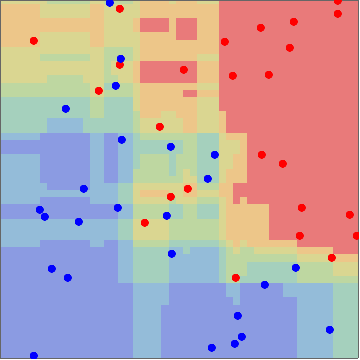
\includegraphics[height=0.35\textheight]{random_forest.png}
\end{figure}

Случайный лес (\texttt{Random Forest}\cite{randomforest}) --- модель машинного
обучения, основанная на применении ансамбля деревьев принятия решения, где
каждое дерево обучается независимо от остальных. Итоговый результат получается
как среднее (взвешенное среднее) по все ответам отдельных деревьев. Так как
каждое дерево разбивает пространство на прямоугольные области, где оно
возвращает одинаковые значения, то итоговый лес является пересечением всех таких
разбиений~\cref{random_forest}. Случайный лес называется регрессионным, если он
используется для решения задач предсказания некоторого численного значения.

Для обучения регрессионного леса, исходные входные данные разбиваются на случайные
подвыборки с повторениями. После чего, на каждой выборке обучается отдельное
дерево принятия решений. Так же применяется метод \texttt{feature
bagging}~\cite{bagging}, где деревья обучаются не на полном наборе признаков,
а только на случено выбранном его подмножестве.

\section{Постановка задачи}

В данной работе рассматривается задача \emph{оптимизации случайного
регрессионного леса}.

Оптимизация --- задача нахождения экстремума (минимума или максимума) целевой
функци в некоторой области. Так как случайный лес разбивает пространство на
конечное число областей, то имеет место случай комбинаторной
оптимизации~\cite{optimize}.

Постановка Задачи: дан заранее обученный случайный лес. Необходимо найти области
пространства признаков в которых данный случайный лес возвращает свои
максимальное/минимальное значения.

\section{Актуальность поставленной задачи}

Частое практическое применение случайного регрессионного леса это  предсказание
некоторой неизвестной функции по набору её значений. Это предсказание может
применяться в качестве суррогатной модели в других алгоритмах машинного
обучения. Одним из примеров такого применения является бесовская оптимизация.

Байесовская оптимизация (Bayesian Optimization),~\cite{bayes1}. Данный
метод строит регрессионную модель на основе результатов запусков настраиваемого
алгоритма. Эта модель позволяет предсказать, где достигается минимум
оптимизируемой функции. Для уточнения предсказаний вблизи некоторой точки,
настраиваемый алгоритм запускается снова, позволяя до-обучить модель.

Для выбора точек, в которых необходимо уточнить модель, можно воспользоваться
понятием \emph{ожидаемого улучшения} (\emph{expected improvement,
EI})~\cite{globalopt}, которое также известно как \emph{верхняя доверительная
граница} Гауссовского процесса (\emph{upper confidence bound,
UCB})~\cite{gaussbandit}.

Частным случаем Байесовской оптимизации является Последовательная Оптимизация,
Основанная на Модели (Sequental Model-Based Optimization, SMBO)~\cite{smac}. Ее
частным случаем является алгоритм Sequential Model-based Algorithm Configuration
(SMAC)~\cite{elf}. Этот алгоритм нам особо интересен, так как в его авторской
реализации применяется случайный лес в качестве регрессионной модели.

Далее а работе произведено исследование эффективности предложенных методов
решения поставленной задачи в приложении на описанный выше метод алгоритм
SMAC.\@

\section{Существующие решения}

Так как функция задаваемая случайным лесом является трудно обратимой,
в настоящее время методы для её оптимизации не рассматривают внутреннюю
структуру случайного леса, а применяются общие методы для оптимизаций суррогатных
функции.

В данном случае основные подходы это:
\begin{enumerate}
    \item Случайный поиск~\cite{random} --- выдирается случайная точка в пространстве,
    вычисляется значение функции в данной точке. Если полученный ответ лучше
    найденного ранее, то значение ответа обновляется.
    \item Локальный поиск --- поиск начинается из заданной точки, и на каждом шаге
    алгоритм переходит в соседнюю с лучшим значением оптимизируемой функции. Поиск
    останавливается при достижении локального экстремума или по истечении
    установленного времени.
\end{enumerate}

Также применяется комбинация этих двух алгоритмов, где производится локальный
поиск из набора случайных стартовых точек~\cite{local}.

\section{Метод имитации отжига}

Популярным методом для решения задач оптимизации является метод имитации
отжига~\cite{od}. Это общий алгоритмический метод решения задачи глобальной
оптимизации, особенно дискретной или комбинаторной. Основной идеей алгоритма,
является имитация физического процесса, происходящего при отжиге металлов,
откуда алгоритм и берет своё название.

Алгоритм производит случайные мутации по переходу из рассматриваемой точки
в соседнюю. При этом, переход в точку с худшим значением целевой функции
осуществляется с вероятностью, постепенно убывающей в соответствии с понижением
температуры:

\[
P(x_i \to x_{i+1}) =
\begin{cases}
    1,                                                  & F(x_i+1) > F(x_i) \\
    \exp \left(-\dfrac{F(x_{i+1})-F(x_i)}{T_i}\right),  & F(x_i+1) \geqslant F(x_i)
\end{cases}
\]

Где $P(x_i \to x_{i+1})$ --- вероятность события перехода в из точки $x_i$
в точку $x_{i+1}$. $F$ --- целевая функция. $T_i > 0$ --- убывающий
температурный параметр.

Основное преимущество данного алгоритма по сравнению с похожими методами
(локальный поиск) --- это случайность при переходе в следующее значение. Что
позволяет избегать остановки алгоритма в локальных экстремумах функции.

\section{Метод ветвей и границ}

Метод ветвей и границ (\texttt{branch and bound}~\cite{branch}) --- ещё один
подход для решения задач комбинаторной оптимизации. Основывается на методе
полного перебора, с отсечением тех вариантов, которые гарантированно не могут
улучшить найденное значение.

Основная идея метода заключается в том, что при некоторых ограничениях на
параметры целевой функции можно оценить её возможные значения. Тем самым можно
не перебирать те границы в которых гарантированно нет максимума функции, а те
границы в которых он потенциально может быть разбиваются на меньшие участки
и процесс повторяется.

Так как метод является вариацией полного перебора, то его эффективность сильно
зависит от качества оценки функции в заданных границах и правильного подбора
этих границ.

\chapterconclusion

В данной главе произведено теоретическое введение в модель машинного обучения
''случайный регрессионный лес'' и входящих в неё компонентов. Поставлена задача,
решаемая в данной работе. 

Также описаны и рассмотрены характеристики алгоритмов оптимизации, которые
используются на практике в данный монумент, и методы использованные в работе.

В данной работе предложен и реализован метод ветвей и границ для оптимизации
функции заданной случайным лесом.

\chapter{Предложенные алгоритмы оптимизации случайного леса}

\section{Метод имитации отжига}

Все пространство разбивается на прямоугольную сетку, где каждая прямая
соответствует одной из границ разветвлений в вершине одного из деревьев. Для
всех прямых также храниться информация в каком дереве происходит разветвление по
данной границе. Важно заметить, что по одному и тому же разбиению могут
происходить несколько вершин в разный деревьях или в одном дереве.

В процессе имитации отжига выполняются случайные мутации по переходу в соседнюю клетку сетки.
Так как при таком переходе пересекается лишь одна граница, для получения нового
значения достаточно пересчитать лишь те деревья в которых есть эта граница, то
есть те, что был и сохранены ранее для границ.

\subsection{Теоретическое сравнение}

\begin{itemize}
    \item \textbf{Преимущество метода:} Константное время работы, не
    зависящие от внутренней сложности устройства конкретных деревьев в лесе.
    \item \textbf{Недостатки метода:} Так как это общий метод оптимизации функции, то
    данный метод не использует внутреннею структуру случайного леса,
    а рассматривает его как 'чёрный ящик'. Кроме этого, часто переход в соседнюю
    клетку происходит по границе, которая не влияет на текущее значение,
    следовательно оно не изменяется. В итоге алгоритму приходится делать большое
    количество не существенный мутаций, что усложняет его работу.
\end{itemize}

\subsection{Результаты}
На практике данный метод не показал желаемых результатов, и было принято решение
отказаться от него в пользу более эффективных. Возможно существуют более эффективные
реализации метода имитации отжига, не рассмотренные в данной работе.


\section{Метод ветвей и границ}

В алгоритме применяется полный перебор всех поддеревьев. В процессе перебора
поддерживается следующий инвариант: все рассматриваемые поддеревья имеют не
пустое пересечение. Тем самым в каждый момент времени рассматривается некоторая
область в виде n-мерного прямоугольника. На каждом шаге перебора, то есть
переходе из вершины в левого или правого ребёнка, эта область разрезается на две
части по границе из вершины, в которой был совершён шаг.

Тем самым границей на функцию является рассматриваемый в конкретный момент
времени прямоугольник. Для оценки максимума и минимума функции в этой области
для каждой вершины посчитано максимальное значение в её поддереве. Так как
случайный лес возвращает среднее значение всех деревьев, то в данной области лес
не может вернуть значение больше (меньше) чем среднее по всем достижимым
максимумам (минимумам) в поддеревьях, задающих эту область. Что позволяет нам
получить необходимые ограничения на оптимизируемую функцию.

В итоге алгоритм не будет рассматривать поддеревья которые гарантированно не
превосходят ранее найденный ответ.

\subsection{Эвристика}

Основная эвристическая оптимизация --- перебирать сначала те поддеревья,
в которых разница между левым и правым детьми максимальна.

\[
    i = \arg \max_{v \in trees}(|value[v.left] - value[v.right]|)
\]

Идея основывается на предположении, что после обхода поддерева первого ребёнка
в такой паре. Из-за максимальной разницы между ними следует большая вероятность
того, что алгоритму не придётся рассматривать поддерево второго ребёнка.

\subsection{Нахождение приближенного значения}

Для поиска ответа с заданной точностью применена следующая оптимизация. Алгоритм
не рассматривает те поддеревья которые гарантированно не превосходят ранее
найденный ответ на больше чем заданное $\alpha$.

\[
    value[v] < \alpha current
\]

Это позволяет находить ответ отличающийся от истинного не более чем на заданную
точность, потому что если найденный ответ отличается больше, то не было
рассмотрено его поддерево, что невозможно так как возможный максимум в нем
больше.

\subsection{Уточнение границ в поддереве}

Заметим, что максимум в поддереве может не пересекаться с областью, которую
рассматривает алгоритм в конкретный момент. Из-за этого алгоритм может
перебирать поддеревья, максимум в которых заведомо не достижим.

Чтобы это исправить для каждого дерева принятия решений посчитан отсортированный
список всех его листьев. Данный список строиться путём последовательного слияния
списков детей в каждой вершине, что асимптотически добавляет $O(N \log{N})$
времени к предподсчету алгоритма, где $N$ --- количество листьев в дереве.

Так как на каждом шаге алгоритма новая полученная область строго включается
в старую, в таком отсортированном списке возможный максимум в поддереве строго
движется вперёд. В итоге за добавление линейного времени на каждый спуск
возможно оценить максимум в поддереве, пересекающийся с текущей рассматриваемой
областью.

\subsection{Оптимизация в заданной области}

Отметим, что в данной реализации алгоритма, можно задать начальные ограничения
на пространство признаков, в котором происходит поиск максимума или минимума.
Что позволяет решать задачу оптимизации не на всем пространстве, а в конкретной
области.

\chapterconclusion

В данной главе предложены два метода оптимизации случайного регрессионного леса
применённые в работе, и как эти методы применяются для решения задачи,
поставленной в работе. Изложены применённые оптимизации к этим методам и детали
реализации в конкретной работе.

Если метод отжига является идейным продолжении применяющихся сейчас на практике
решений поставленной задачи, то метод ветвей и границ является кардинально новым
подходом к решению оптимизации случайного леса.

При экспериментальном исследовании, от метода имитации отжига было принято решение
отказаться в пользу метода ветвей и границ.

\chapter{Экспериментальное исследование предложенных подходов}\label{chap:third}

\section{Реализация алгоритма}\label{sec:impl}

За основу была взята реализация алгоритма случайного регрессионного леса
\texttt{RandomForestRegressor} из \texttt{Python} библиотеки
\texttt{sklearn-kit}\footnote{\url{http://scikit-learn.org/}}. 

К стандартному функционалу леса добавлена функция вычисления максимума или
минимума на всем пространстве или же заранее заданном его подпространстве,
с возможностью выбора алгоритма оптимизации (случайный поиск, метод ветвей
и границ, метод ветвей и границ с применением эвристик), допустимой погрешности
(для алгоритмов на основе ветвей и границ) и количества итераций (для алгоритмов
на основе случайного или локального поиска). 

\section{Параметры и метод тестирования}\label{sec:test}

Для обучения случайных лесов применялись общедоступные наборы данных из открытой
базы данных OpenML, их параметры приведены в таблице~\ref{tab_datasets}.

\begin{center}
    \begin{table}[H]
    \caption{Таблица с параметрами использованных наборов данных}\label{tab_datasets}
        \begin{tabular}{|l|l|l|}

\hline

название        & элементы  & признаки \\

\hline

diabetes        & 442    & 9     \\
boston          & 506    & 12    \\
autoPrice       & 159    & 16    \\
wisconsin       & 194    & 33    \\
strikes         & 625    & 7     \\
kin8nm          & 8192   & 9     \\
house\_8L       & 22784  & 9     \\
house\_16H      & 22784  & 9     \\
mtp2            & 274    & 1143  \\

\hline

\end{tabular}

    \end{table}
\end{center}

В работе было произведено сравнение следующих алгоритмов следующие алгоритмы: 

\begin{enumerate}
        \item Метод ветвей и границ 
        \item Метод ветвей и границ с погрешностью $<5\%$
        \item Случайный
        \item Отжиг
        \item Метод ветвей и границ с применением эвристики
        \item Метод ветвей и границ с применением эвристики и с погрешностью $<5\%$
        \item Метод ветвей и границ с применением эвристики и с погрешностью $<15\%$
\end{enumerate}

На каждом наборе параметров (то есть: набор данных, количество деревьев,
максимальная глубина) обучалось 10 лесов с разными случайными начальными
значениями, после чего на каждом запускались все рассматриваемые алгоритмы
оптимизации. По результатам запусков вычислялось математическое ожидание
и среднеквадратическое отклонение времени работы алгоритма. Так же вычислялась
относительная погрешность результата по следующей формуле:

\[
    \sigma = \frac{Max_{correct} - Max_{found} + Min_{correct} - Min_{found}}
    {Max_{correct} - Min_{correct}}
\]

\section{Результаты}\label{sec:results}

\subsection{Время работы}

На графиках (\cref{timeeasy,timetrees,timebig}) изображено сравнение
рассматриваемых алгоритмов по времени их работы в разных условиях. Графики
сгруппированы по характеру начальной выборки, на которой обучался целевой лес,
а так же по количеству деревьев в обучаемом лесу, так как это два основных
параметра влияющих на качество и время работы оптимизации. Пустой столбец на
графике с только одной линией погрешности означает, что алгоритм работал не
целесообразно долго и был остановлен по достижении ограничения на время ($600$
сек.).

\begin{figure}[H]
    \caption{Сравнение времени работы на простых выборках с небольшим
    количеством деревьев ($<50$)}\label{timeeasy}
    \timeeasy{0.90\textwidth}{0.35\textheight}
\end{figure}

Как видно из графика \cref{timeeasy} применение эвристической оптимизации
существенно сокращает время работы алгоритма, в случае не большого количества
неглубоких деревьев. Это происходит, потому что в таком случае первый несколько
найденных ответов приводят к отсечению большого количества поддеревьев, которые
алгоритм не будет рассматривать.

\begin{figure}[H]
    \caption{Сравнение времени работы на простых выборках с большим количеством
    деревьев ($>50$)}\label{timetrees}
    \timetrees{0.75\textwidth}{0.45\textheight} 
\end{figure}

На графике \cref{timetrees} видно, что увеличение количества деревьев, сильно
сказывается на времени работы алгоритмов. Случайный алгоритм очевидно
асимптотически имеет линейную зависимость времени работы, от количества
деревьев, так как он производит константное количество вызовов случайного леса.
В то время как метод ветвей и границ, так как является полным перебор,
потенциально имеет экспоненциальную зависимость. Но на графике видно, что
добавление погрешности в таком случае сильно уменьшает время работы. Это
происходит, потому при большом количестве деревьев, существует множество наборов
поддеревьев имеющих близкие к друг-другу значения потенциальных максимума
и минимума. Особенно хорошо это заметно на наборе данных diabites
(см.~\cref{tab_datasets}) с $50$ деревьями

\begin{figure}[H]
    \caption{Сравнение времени работы на сложных начальных выборках}\label{timebig}
    \timebig{0.80\textwidth}{0.40\textheight} 
\end{figure}

График \cref{timebig} демонстрирует, что сложность изначальной выборки,
а следовательно глубина обученных деревьев, влияет только на время работы
алгоритмов перебора, так как случайный алгоритм не зависит от внутренней
структуры конкретных деревьев леса. При этом в таком случае применение
оптимизации с погрешностью, хоть и даёт выигрыш по времени, но не такой
заметный, как в случае с большим количеством деревьев, так как здесь сложность
работы вызывается перебором поддеревьев одного глубоко дерева, а не поддеревьев
разных деревьев леса.

\subsection{Погрешность}\label{sec:error}

На графиках (\cref{erroreasy,errorbig}) изображено сравнение рассматриваемых
алгоритмов по погрешности найденного значения в разных условиях. Графики
сгруппированы по характеру начальной выборки, на которой обучался целевой лес.
На графиках отсутствуют алгоритмы возвращающие точное значение результата (метод
ветвей и границ без погрешности), так как их погрешность равна $0$.

\begin{figure}[H]
    \caption{Сравнение погрешности работы}\label{erroreasy}
    \erroreasy{0.9\textwidth}{0.45\textheight}
\end{figure}

Как видно из графика \cref{erroreasy} алгоритмы полного перебора стабильно
находят значение точнее заявленной погрешности. Это происходит потому, что
заданное значение погрешности применяется для отсеивания поддеревьев, которые
гарантированно не улучшают найденное значение экстремума. Но так как мы
используем крайнюю оценку возможных значений в поддереве, то на практике это
значение редко достигается и реальное улучшение достижимое в пропущенном
поддереве оказывается сильно меньше оценочного значения. Так же на графике видно
не эффективность реализованного метода отжига. В следствии того, что он
затрачивает большее время на одну итерацию, то при равном ограничении по времени
отжиг оказывается менее эффективным по сравнению с случайным поиском.
В результате, было принято решение отказаться от рассмотрения алгоритма имитации
отжига далее в работе.

\begin{figure}[H]
    \caption{Сравнение погрешности работы на выборках с большим количеством
    признаков.}\label{errorbig}
    \errorbig{0.8\textwidth}{0.45\textheight}
\end{figure} 

График \cref{errorbig} показывает абсолютную не применимость алгоритмов
случайного и локального поиска в случаях большого количества признаков (более
$20$ признаков) в изначальной выборке. В то время, как из-за простой внутренней
структуры алгоритм перебора находит точное значение, даже при большой заданной
погрешности. Особенно хорошо это демонстрирует выборка с более $1000$ признаками
(mtp2 см.~\cref{tab_datasets})

\begin{figure}[H]
    \caption{Сравнение времени работы в зависимости от
    погрешности}\label{error_to_time}
    \errortotime{0.9\textwidth}{0.6\textheight} 
\end{figure}

Чтобы лучше продемонстрировать эффективность описанной раннее оптимизации поиска
с погрешностью. Было произведено сравнение зависимости времени работы алгоритма,
от заданной погрешности в применении на случайные леса обученные на 4 разных
выборках:

\begin{enumerate}
    \item diabetes, с 50 обучаемыми деревьями
    \item kin8nm, с 30 обучаемыми деревьями
    \item house8L, с 37 обучаемыми деревьями
    \item house16L, с 20 обучаемыми деревьями
\end{enumerate}

График \cref{error_to_time} демонстрирует обратную экспоненциальную зависимость
времени работы, от заявленной погрешности применяемого алгоритма. Что
подтверждает сделанное ранее предположение.

\section{Экспериментальное исследование предложенных методов в применении на
практике}\label{sec:test_smac}

Было проведено сравнения модифицированной версии алгоритма SMAC с подбором новых
кандидатов, применяя разработанный алгоритма поиска минимума в случайном лесу.
Тестирование производилось на подборе гиперпараметров для трёх алгоритмов
квалификации из библиотеки sklearn-kit:

\begin{enumerate}
    \item Random Forest Classifier
    \item Decision Tree Classifier
    \item SGD Classifier
\end{enumerate}

Для каждого алгоритма был произведён подбор гиперпараметров применением сначала
оригинального алгоритма SMAC, а затем модифицированной версией алгоритма
с использованием оптимизации случайного леса. На каждой начальной выборке
производилось $10$ запусков SMAC с разными случайными ключами, после чего
вычислялось среднее и погрешность по всем запускам. Для оценки точности
предложенных гиперпараметров, применялась перекрёстная проверка с разбиением
исходной выборки на $5$ равных частей.

Сравнение производилось с двумя алгоритмами использованными в automl реализации
SMAC:\@ случайный поиск и случайный поиск в сочетании локальным поиском. Важно
отметить, что второй алгоритм, хоть и обычно достигает более высоких оценок
точности чем случайный поиск, но это достигается ценой длительного времени
работы. Время работы предложенного алгоритма с применением оптимизации
случайного леса (и случайного поиска) не существенно по сравнению со временем
обучения целевой модели. Так как, в данной реализации применяется не большой
регрессионный лес (10 деревьев), обученный на не большой выборке (количество
запусков целевого алгоритма). Как было продемонстрировано выше в работе, в таком
случае алгоритм крайне эффективен.

\begin{table}[H]
\centering
\caption{Сравнение работы оригинального алгоритма SMAC и с применением оптимизации
случайного леса, выделены те значения где предложенная модификация достигает
лучшей оценки точности.}\label{smacgeneral}
\smacgeneral
\end{table}

В \cref{smacgeneral} продемонстрированы результаты описанного выше
экспериментального исследования. Видно, что в некоторых случаях оба варианта
алгоритма достигают одинаковой оценки точности целевого алгоритма, но можно
заметить, что в таких случаях алгоритм имеет крайне низкий разброс результатов,
а значит, оба алгоритма с большой вероятностью находят лучшую возможную
конфигурацию для данного случая. В случаях с большой погрешностью, предложенная
модификация стабильно достигает лучших оценок точности по сравнению
с оригинальным алгоритмом.

Для тестирования подбирались гиперпараметры для дерева принятия решений. Этот
выбран исходя из следующих соображений:

\begin{itemize}
    \item Быстрый и лёгкий алгоритм, не требующий сложных и длительный вычислений.
    Этот критерий важен, так как целевой алгоритм запускается порядка $1000$ раз за один тест.
    \item Алгоритм требует подбора гиперпараметров, и без этого работает крайне
    не эффективно. (оценка точности $0.2$ со стандартной конфигурацией)
\end{itemize}

\begin{figure}[H]
\caption{Зависимость от размера пространства гиперпараметров}\label{smac_size}
\smacsize{0.6\textwidth}{0.4\textheight}
\end{figure}

На графике~\cref{smac_size} изображена зависимость оценки точности целевого
алгоритма от размера пространства гиперпараметров. То есть от количества
различных комбинаций гиперпараметров. Для этого изначальный набор
гиперпараметров был искусственно ограничен, на соответствующий коэффициент по
всем параметрам. Для каждой выборки было произведено всего по $4$ эксперимента по
причине длительной работы алгоритма SMAC, особенно в его оригинальной
реализации. Изображено по две линии одного цвета для каждого набора данных.
Верхняя линия соответствует предложенной модификации, а нижняя оригинальному
алгоритму. Данный график показывает, что применение предложенного метода
позволяет получать более стабильные результаты при увеличении пространства
гиперпараметров.

\begin{figure}[H]
\caption{Зависимость от размера пространства гиперпараметров}\label{smac_count}
\smaccount{0.6\textwidth}{0.4\textheight}
\end{figure}

На графике~\cref{smac_count} изображена зависимость оценки точности целевого
алгоритма от ограничения на количество запусков целевого алгоритма. Линии на
графике группированы по тому же принципу, что и в предыдущем. График
демонстрирует, что основное преимущество предложенного в работе подхода --- это
сокращение необходимого количества запусков целевого алгоритма, для достижения
той же оценки точности предсказываемого результата. С учётом того, что при этом
алгоритм оптимизации работает значительно меньшее время, предложенный метод
затрачивает значительно меньшее время для достижения эквивалентных результатов.

\chapterconclusion{}

Сначала было произведён вспомогательный сравнительный анализ работы описанных
раннее в работе методов и подходов к оптимизации функции заданной случайным
регрессионным лесом, в ходе которого хорошо заметно превосходящая эффективность
метода ветвей и границ, как в плане времени работы, так и достигаемой при этом
погрешности результата.

Показано и объяснено влияние количества деревьев и глубины деревьев
в оптимизируемой лесу на время и погрешность работы исследуемых алгоритмов.
Произведён анализ зависимости времени работы методов полного перебора от
заданной допустимой погрешности.

После этого метод ветвей и границ был применён в реализации алгоритма SMAC для
оптимизации его регрессионной модели (случайного леса). Разработанный алгоритм
демонстрирует более высокие оценки точности целевой модели при одинаковом наборе
параметров и равном временном бюджете. При этом, чем меньше ограничение по
времени работы и количеству запусков, тем больше заметна разница между
рассматриваемыми алгоритмами.


%% Макрос для заключения. Совместим со старым стилевиком.
\startconclusionpage{}
В данной работе был предложен новый подход к решению задачи оптимизации функции
заданной случайным лесом.

Было проведено масштабное сравнение предложенных методов и существующих сейчас
алгоритмов. В результате которого метод ветвей и границ был принят как самый
эффективный. Так же проведено сравнение его работы при различных настраиваемых
параметрах и в приложении на по разному обученные случайные леса.

После чего этот метод был реализован в применении на практической задачи выбора
модели и настройки её гиперпараметров. Предложенный алгоритм продемонстрировал
статистически значимые лучшие результаты. Он может успешно применяться в любых
случаях оптимизации леса.

Таким образом, цель достигнута и все задачи выполнены.

\printmainbibliography%

\end{document}
